\documentclass[border=10pt]{standalone}
\usepackage{pgfplots}
\pgfplotsset{compat=1.18}
\begin{document}
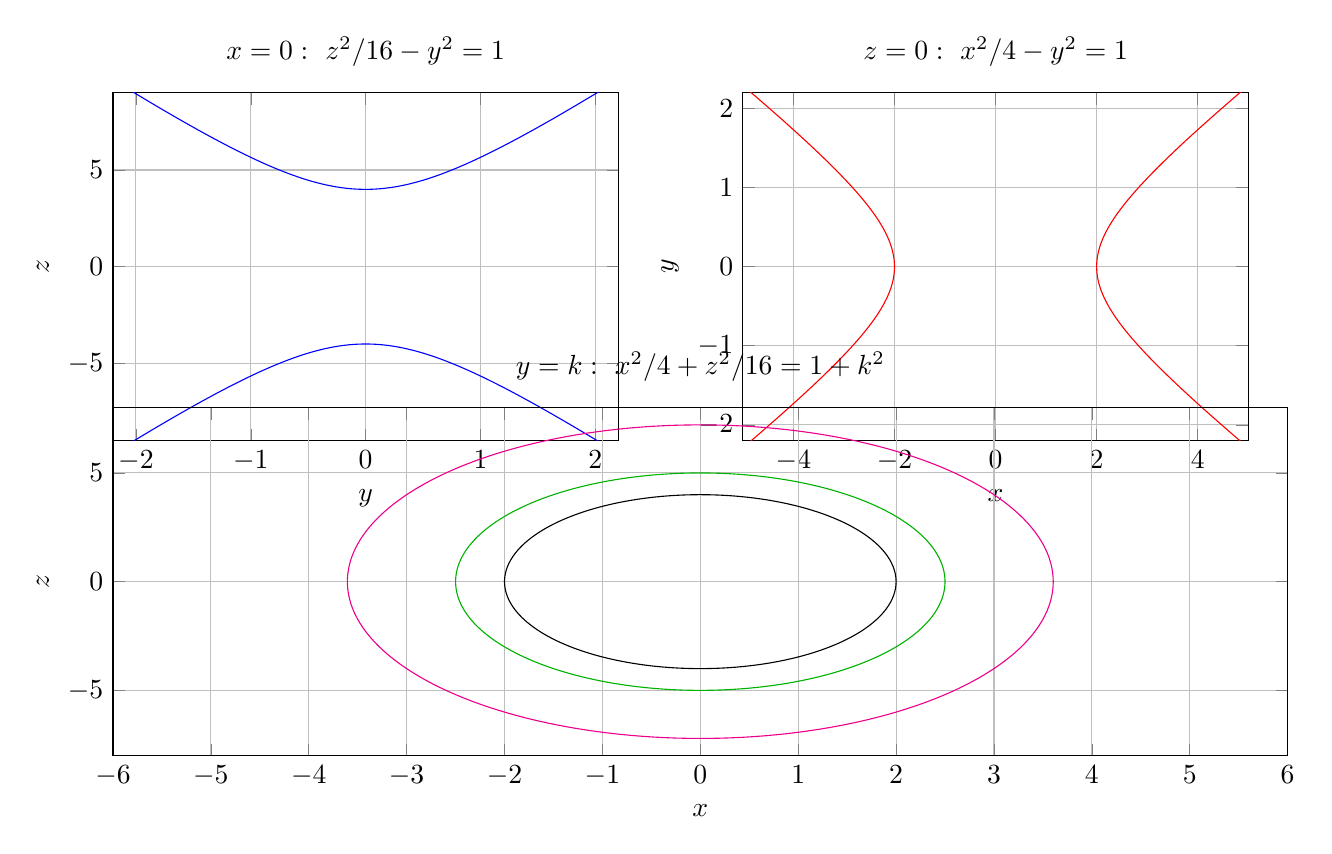
\begin{tikzpicture}
\begin{axis}[
    width=8cm, height=6cm, at={(0cm,4cm)},
    xlabel={$y$}, ylabel={$z$}, grid=major,
    title={$x=0:\ z^2/16-y^2=1$},
    xmin=-2.2, xmax=2.2, ymin=-9, ymax=9
]
\addplot[blue, domain=-2:2, samples=200] ({sinh(x)}, {4*cosh(x)});
\addplot[blue, domain=-2:2, samples=200] ({sinh(x)}, {-4*cosh(x)});
\end{axis}

\begin{axis}[
    width=8cm, height=6cm, at={(8cm,4cm)},
    xlabel={$x$}, ylabel={$y$}, grid=major,
    title={$z=0:\ x^2/4-y^2=1$},
    xmin=-5, xmax=5, ymin=-2.2, ymax=2.2
]
\addplot[red, domain=-2:2, samples=200] ({2*cosh(x)}, {sinh(x)});
\addplot[red, domain=-2:2, samples=200] ({-2*cosh(x)}, {sinh(x)});
\end{axis}

\begin{axis}[
    width=16.5cm, height=6cm, at={(0cm,0cm)},
    xlabel={$x$}, ylabel={$z$}, grid=major,
    title={$y=k:\ x^2/4+z^2/16=1+k^2$},
    xmin=-6, xmax=6, ymin=-8, ymax=8
]
\addplot[black, domain=0:360, samples=200] ({2*cos(x)}, {4*sin(x)});
\addplot[green!70!black, domain=0:360, samples=200] ({2*sqrt(1+0.75^2)*cos(x)}, {4*sqrt(1+0.75^2)*sin(x)});
\addplot[magenta, domain=0:360, samples=200] ({2*sqrt(1+1.5^2)*cos(x)}, {4*sqrt(1+1.5^2)*sin(x)});
\end{axis}
\end{tikzpicture}
\end{document}